\documentclass{math201}

\usepackage[backref]{hyperref} 
\hypersetup{hidelinks}
\usepackage{bookmark}

% =============================================
% Part 0 信息
% =============================================

\mathsetup{
  % 学生姓名
  student = {},
  % 学号
  student-id = {},
  % 院系
  experiment = {数码管显示控制},
  % 专业年级
  discipline = {集成电路设计与集成系统},
  % 日期
  date = {\today},
}

\begin{document}

% =============================================
% Part 1  封面
% =============================================

\makecover

% =============================================
% Part 2 主文档
% =============================================

\section{实验内容}

通过DSP的通用输入输出多路复合器GPIO来控制开发板上数码管的显示。

\section{实验内容}

(注:实验板上的数码管是共阳数码管)

\subsection{GPIO的寄存器}

对于 DSP 输入/输出引脚的操作,都是通过对寄存器的设置来实现的。
例如,选择某个引脚是作外设功能引脚还是作通用数字I/O口;
当引脚作为通用数字I/O口时,是作输入还是作输出;
如何使其输出高电平或者低电平;
如何使其引脚电平翻转;
如何知道引脚上的电平是高或者是低,这些都是通过对GPIO寄存器的操作来实现的。

GPIO的寄存器分成了两大类:
一类是控制寄存器,主要由功能选择控制寄存器GPxMUX,方向控制寄存器GPxDIR,输入限定控制寄存器GPxQUAL组成,其巾x代表A、B、D、E、F或者是G;
另一类是数据寄存器,主要由数据寄存器GPxDAT、置位寄存器GPxSET、清除寄存器GPxCLEAR和取反寄存器GPxTOGGLE组成,如图一所示。

\begin{figure}[H]  
    \centering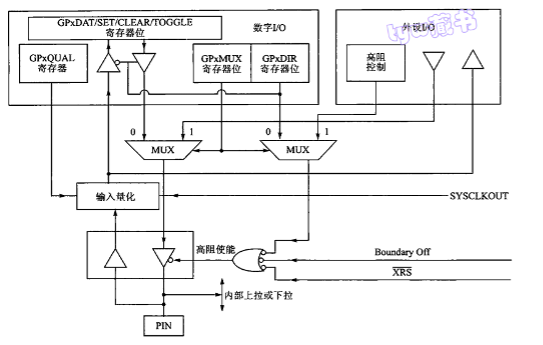
\includegraphics[width=0.8\linewidth]{Picture1.png}  
    \caption{GPIO多路功能复用的原理}     
    \label{img01}   
\end{figure}

\subsection{实验板的LED连接图}

电路原理图如图2所示,七段数码管由A--F控制数字显示,DP为小数点显示,连接至2812的PB0---PB6 ,DIG1---DIG6控制数码管的开关,DIG1---DIG6由三极管开关电路实现高低电平转换,2812的PB8---PB13负责控制开关电路。

\begin{figure}[H]  
    \centering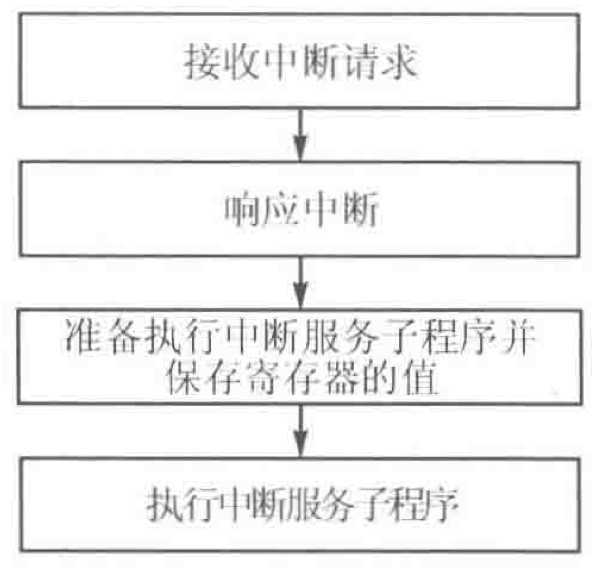
\includegraphics[width=0.8\linewidth]{Picture2.png}  
    \caption{2812数码管连接图}     
    \label{img02}   
\end{figure}

\section{实验步骤}

\subsection{编写代码}

下面是需要在给出代码上进行修改的部分。

Macro\_definition.h

\inputminted[
    frame=lines,
    framesep=2mm,
    baselinestretch=1.2,
    fontsize=\small,
    linenos
]{C++}{code/Macro_definition.h}

num.h, 这是7段数码管显示的代码,控制一下亮暗就行,需要补充0-9数字的显示。

\inputminted[
    frame=lines,
    framesep=2mm,
    baselinestretch=1.2,
    fontsize=\small,
    linenos
]{C++}{code/num.h}

\subsection{编译调试}

\begin{figure}[H]  
    \centering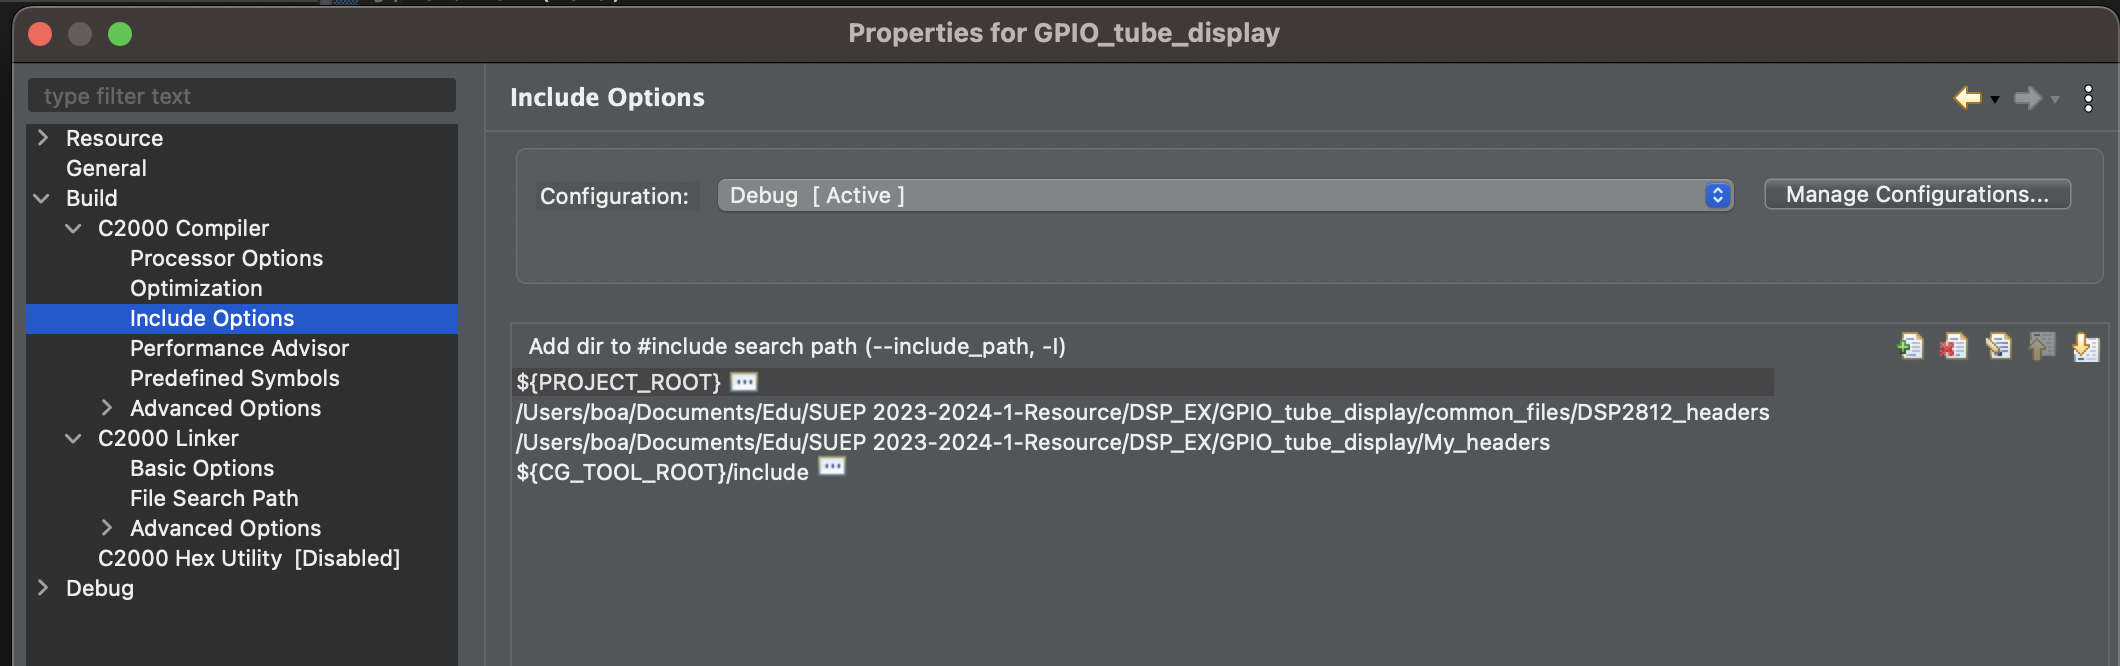
\includegraphics[width=0.8\linewidth]{edit_include_option.png}  
    \caption{edit include option}     
    \label{img03}   
\end{figure}

\begin{figure}[H]  
    \centering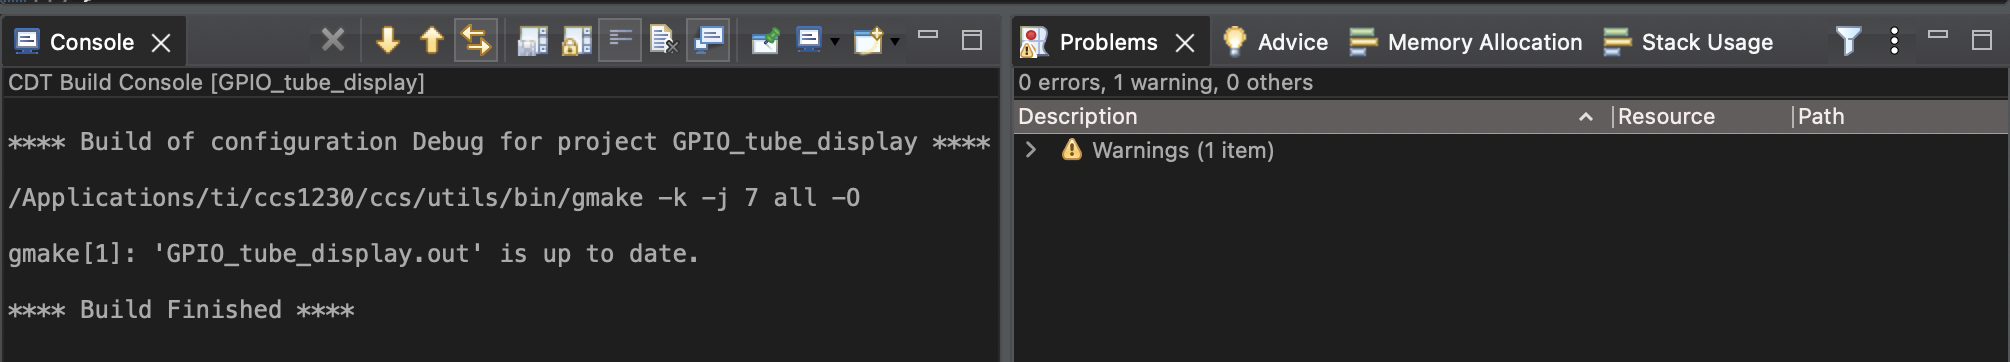
\includegraphics[width=0.8\linewidth]{build.png}  
    \caption{build}     
    \label{img04}   
\end{figure}

\subsection{下载运行、实验现象}

首先,需要添加头文件。

\begin{figure}[H]  
    \centering\includegraphics[width=0.8\linewidth]{debug_phenomenon.jpg}  
    \caption{运行现象}     
    \label{img05}   
\end{figure}

\section{实验小结}

\end{document}
